% mnras_template.tex
%
% LaTeX template for creating an MNRAS paper
%
% v3.0 released 14 May 2015
% (version numbers match those of mnras.cls)
%
% Copyright (C) Royal Astronomical Society 2015
% Authors:
% Keith T. Smith (Royal Astronomical Society)

% Change log
%
% v3.0 May 2015
%    Renamed to match the new package name
%    Version number matches mnras.cls
%    A few minor tweaks to wording
% v1.0 September 2013
%    Beta testing only - never publicly released
%    First version: a simple (ish) template for creating an MNRAS paper

%%%%%%%%%%%%%%%%%%%%%%%%%%%%%%%%%%%%%%%%%%%%%%%%%%
% Basic setup. Most papers should leave these options alone.
\documentclass[a4paper,fleqn,usenatbib]{mnras}

% MNRAS is set in Times font. If you don't have this installed (most LaTeX
% installations will be fine) or prefer the old Computer Modern fonts, comment
% out the following line
%\usepackage{newtxtext,newtxmath}
% Depending on your LaTeX fonts installation, you might get better results with one of these:
%\usepackage{mathptmx}
%\usepackage{txfonts}

% Use vector fonts, so it zooms properly in on-screen viewing software
% Don't change these lines unless you know what you are doing
\usepackage[T1]{fontenc}
\usepackage{ae,aecompl}

%%%%% AUTHORS - PLACE YOUR OWN PACKAGES HERE %%%%%

% Only include extra packages if you really need them. Common packages are:
\usepackage[dvipdfmx]{graphicx}	% Including figure files
\usepackage{amsmath}	% Advanced maths commands
\usepackage{amssymb}	% Extra maths symbols
\usepackage{multicol}
\usepackage{siunitx}
\usepackage{bmpsize}
\usepackage[anythingbreaks]{breakurl}
\usepackage{subfig}
\usepackage{fancyvrb}
\usepackage{hyperref}


\def\startdata{\if@table@not@headed\kill\caption{\\%
    \@tablecaption}\endhead\hline\endfoot%
  \fi%
}

\def\enddata{% 
 \crcr 
 \noalign{\vskip .7ex}% 
 \before@enddata 
 \endtabular 
 \setbox\pt@box\lastbox 
 \pt@width\wd\pt@box\box\pt@box 
}% 


\newcommand{\aprx}{\raise.17ex\hbox{$\scriptstyle\sim$}}

%%%%%%%%%%%%%%%%%%%%%%%%%%%%%%%%%%%%%%%%%%%%%%%%%%

%%%%% AUTHORS - PLACE YOUR OWN COMMANDS HERE %%%%%

% Please keep new commands to a minimum, and use \newcommand not \def to avoid
% overwriting existing commands. Example:
%\newcommand{\pcm}{\,cm$^{-2}$}	% per cm-squared

%%%%%%%%%%%%%%%%%%%%%%%%%%%%%%%%%%%%%%%%%%%%%%%%%%

%%%%%%%%%%%%%%%%%%% TITLE PAGE %%%%%%%%%%%%%%%%%%%

% Title of the paper, and the short title which is used in the headers.
% Keep the title short and informative.
\title[SPIDERMAN]{SPIDERMAN: an open source code to model phase curves and secondary eclipses.}

% The list of authors, and the short list which is used in the headers.
% If you need two or more lines of authors, add an extra line using \newauthor
\author[T. Louden, L. Kreidberg]{Tom Louden$^{1}$\thanks{E-mail: t.m.louden@warwick.ac.uk} and Laura Kreidberg$^{2}$\\
$^{1}$Department of Physics, University of Warwick, Coventry, CV4 7AL, UK\\
$^{2}$Harvard-Smithsonian Center for Astrophysics, Cambridge, MA 02138, USA}

% These dates will be filled out by the publisher
\date{Accepted XXX. Received YYY; in original form ZZZ}

% Enter the current year, for the copyright statements etc.
\pubyear{2016}

% Don't change these lines
\begin{document}
\label{firstpage}
\pagerange{\pageref{firstpage}--\pageref{lastpage}}
\maketitle

% Abstract of the paper
\begin{abstract}

Presenting \textsc{spiderman}, a fast code for calculating exoplanet phase curves and secondary eclipses with arbitrary surface brightness distributions.

Using a geometrical algorithm, the code solves exactly the area of sections of the disc of the planet that are occulted by the star. The code is written in C and optimised to run quickly, with no loss in precision. Approximately 1000 models can be generated per second with typical parameters, making Markov Chain Monte Carlo analyses practicable. The modular nature of the code allows easy comparison of the effect of multiple different brightness distributions of the dataset.

As a test case we apply the code to archival data on the phase curve of WASP-43b using a physically motivated analytical model for the brightness model. The model provides a good fit to the data, however it overpredicts the temperature of the night-side. We speculate that this could be due to the presence of clouds on the night side of the planet. We also test for variation of the map parameters as a function of wavelength and find no statistically significant correlations.

\textsc{spiderman} is available for download at \url{https://github.com/tomlouden/spiderman}.

\end{abstract}

% Select between one and six entries from the list of approved keywords.
% Don't make up new ones.
\begin{keywords}
%planets and satellites: individual (WASP 43b)---stars: individual (WASP 43)---techniques: spectroscopic---planets and satellites: atmospheres---celestial mechanics---atmospheric effects
\end{keywords}

%%%%%%%%%%%%%%%%%%%%%%%%%%%%%%%%%%%%%%%%%%%%%%%%%%

%%%%%%%%%%%%%%%%% BODY OF PAPER %%%%%%%%%%%%%%%%%%

\section{Introduction}\label{sec:introduction}

Secondary eclipses and phase curves can give direct insight into the thermal transport processes, and when wavelength resolved also give information on the vertical structure of an exoplanet atmosphere. The details of heat transport in the atmosphere will effect how efficiently energy can be transported between the two hemispheres of the planet.

General Circulation Models (GCM's), are currently the state of the art for predicting the wind patters and temperature distributions of the surface of exoplanets \citep[e.g.][]{Showman2008}. An important early prediction of these GCM's was that hot, tidally locked Jupiter's would display significantly offset hotpots. The hotspot offset is the result of fast superotating equatorial winds in the atmosphere that arise from a coupling of planetary scale circulation and day night advection \citep{Showman2011}.

The high equilibrium temperature of Hot Jupiters affords them contrasts with their parents stars of order 0.1\%, making direct detection with current generation instruments feasible. \citet{Deming2005} detected the infrared flux of HD\,209458b by observing the secondary transit of the planet with the MIPS instrument on \emph{Spitzer}. Using the IRAC instrument on \emph{Spitzer}, \citet{Knutson2007b} went on to measure the secondary eclipse of HD\,189733b with high precision, and also show that the system displayed a sinusoidal \emph{phase curve}, caused by the bright regions of the planet rotating into and out of view. Intriguingly, the phase of this sinusoidal curve was significantly offset from the time of secondary eclipse, validating earlier predictions from GCM's. This effect can also be mimicked by a high eccentricity, but \citet{J.deWit2012a} show that this is not the case for HD\,189733b.

There appear to be, broadly, two classes of exoplanet atmospheres with regards to heat transport. Hot Jupiters like HD\,189733b with, relatively low temperatures have highly significant hotspot offsets and efficient day-night redistribution \citep{Knutson2007b}. $\mu$ Andromedae, HD\,179949b and HD\,209458b are all significantly hotter than HD\,189733b and display much higher temperature contrasts between the day and night sides, implying inefficient redistribution of energy. \citep{Harrington2006,Cowan2007,zellem2014}. This behavior can be explained with the results of General Circulation Models \citep{Komacek2015,Komacek2016}

The high velocity winds transporting this energy have been predicted to be on the order of kilometers per second, which would leave a measurable imprint on the spectral absorption lines in the planets atmosphere through Doppler shifting \citep[e.g.][]{Showman2013}, and indeed, this effect has been observed in the transit of HD\,209458b \citep{Snellen2010} and HD\,189733b \citep{Louden2015}. 

\cite{Majeau2012} showed that as well as mapping longitudinally with phase curves, it is possible to get a two dimensional map of the dayside of an exoplanet from the secondary eclipse, provided that there is a non zero impact parameter. This technique works because the inclination of the system results in the occulting limb of the star scanning across the disc of the planet in both longitude and latitude during ingress and egress. The brightness distribution of the planet's permanent dayside will be imprinted on the precise shape of the ingress and egress curves.

When phase curves are spectrally resolved, they can provide an extremely powerful tool for accessing the vertical structure of an exoplanet atmosphere as a function of longitude. \citet{Stevenson2014} use WFC3 on \textsc{HST} to measure the emission spectrum and recover the Temperature-Pressure profile of WASP-43b as a function of phase.

%JWST expectations?

An open source code for calculating both exoplanet eclipses and phase curves in a self consistent way for arbitrary brightness distributions does not currently exist. \textsc{batman} \citep{Kreidberg2015a} is an open source code to model exoplanet primary transits with a fast C-based analytical integrator, making it suitable for use with MCMC's, and has found broad use in the exoplanet community. \textsc{spiderman} is designed to fulfill the same role for secondary eclipses and phase curves, and it is is hoped that it will be of use to the community.

In this paper we first describe the model, and provide a brief overview of the code, and then an example of use on the hot Jupiter WASP-43b.

\section{The model}\label{sec:the model}

\subsection{Analytical integrator}\label{sec:integrator}

In order to accurately calculate both the phase curve and secondary eclipse the code must integrate over the portion of the planet that is facing the observer and is not occulted by the star at each time-step. In order to be general use and ``model agnostic'' the integrator cannot assume any specific properties or symmetries in the brightness distribution. This can be done numerically, by sampling a grid of points on the planets surface and summing those that are visible, but to achieve high precisions a large number of points would need to be sampled, which would be slow and computationally inefficient.

Instead, \textsc{spiderman} uses an analytical integration scheme where the planet is divided into a relatively small number of regions, and the area of each region that is not occulted by the star is calculated exactly through geometry. The average surface brightness of each region is determined by the chosen model and multiplied by the visible area to get the total flux.

\textsc{spiderman} uses a radial co-ordinate system centered on the visible hemisphere of the planet. The planet is defined to have a radius of 1 and the visible disc of the planet is divided into a series of annuli, and then these in turn are separated in theta, see the schematic in figure \ref{fig:schematic}. The number of segments in each annuli are chosen so that the area of every sector is the same. This results in 1 circular segment in the center, then 3 regions in the second annuli and 5 in the third - with the number of segment in the nth annuli being 2n - 1. Using this scheme, dividing the planet n times radially results in a total of n$^2$ integration elements.

\begin{figure}
	\begin{center}
		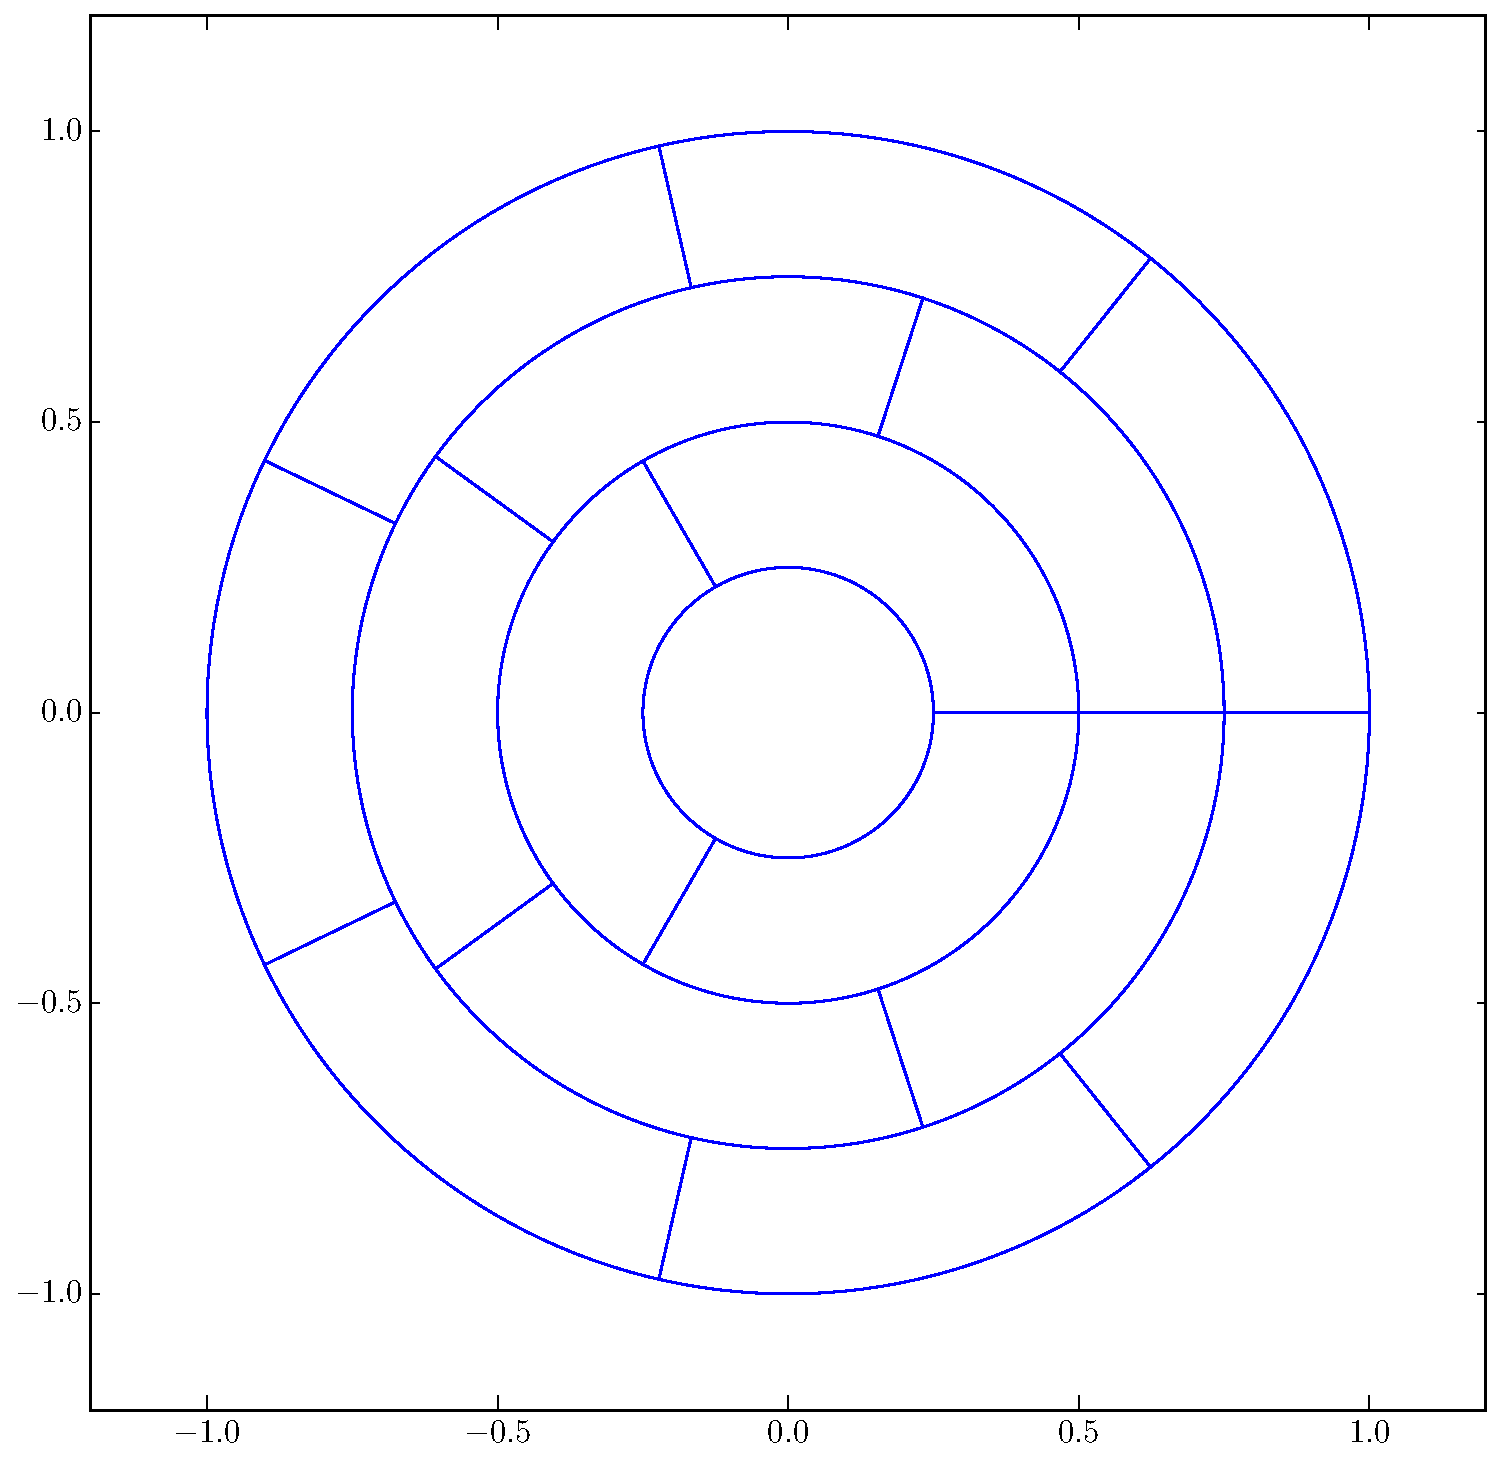
\includegraphics[width=0.8\columnwidth]{img/frame1.pdf}
		\caption{Schematic representation of the planet grid. All sectors are equal area.}
		\label{fig:schematic}
	\end{center}
\end{figure}

Each of the grid segments is a well defined geometric shape for which it is simple to calculate the fraction blocked by the planet passing behind the star, which in the model is represented as an occulting circle.

The area of one of these geometrical segments that has been blocked by the star can always be calculated by breaking the area into a combination of circle segments and triangles, for which the areas are known.

There are a small number of different general ``cases" for the numbers of triangles and segments that must be used, that can be selected based on the number and types of ``collision points" between the planet region and the stellar circle. Therefore, the first step for calculating the occulted area for each segment of the planet is to calculate these collision points. Within \textsc{spiderman} the region boandaries are stored as the radius of the inner and outer arcs, and the $\theta$ angle of the two radial lines.

Finding the collision points between an arc or a line and a circle (the star), if any exist, are trivial and fast to calculate. The code then classifies the geometric ``case" of the collision based on the number of collision points on the 4 boundary sides.

For example, if there are two collision points between the outer arc and the edge of the star, then this falls into the case where the occulted area can be described by the sum of two circular segments. Other cases include larger numbers of components, but can still be described by a small number of circle segments and triangles.

Numerical errors can be introduced by this approach if the brightness distribution changes significantly faster than the area elements, but the size of the elements can be adjusted as necessary by the user, at the cost of computation time.
In practice, we found that dividing the planet into 5 radially (giving 25 total elements) gave sufficient precision for the smoothly varying brightness profile in our WASP-43b test case, and increasing the mesh density beyond this point did not change the results.

Other grid schemes could be defined, for example, if it is decided that the information content is higher in some parts of the planet than others then the grid could be made finer in these regions.

We performed a simple validation check to demonstrate that the integrator is working correctlyl. assuming a uniform brightness distribution, the number of sections that the planet is broken into for the integration should have no impact on the final light-curve.

To test that the integrator is performing correctly we compare the case of a single segment model, i.e., a circle, for which there is a single analytical solution to the area blocked by another circle, to one with 400 segments. In both cases the planet is assumed to have a total luminosity that is 1\% that of the star's.

A lightcurve is calculated for each of these cases, and then the difference is taken. The results of this test can be seen in figure \ref{fig:precision}, where it is clear that there is no difference between the two lightcurves greater than floating point precision (2.22e-16). We therefore consider the geometric integrator of \textsc{spiderman} to be validated.

\begin{figure}
\begin{center}
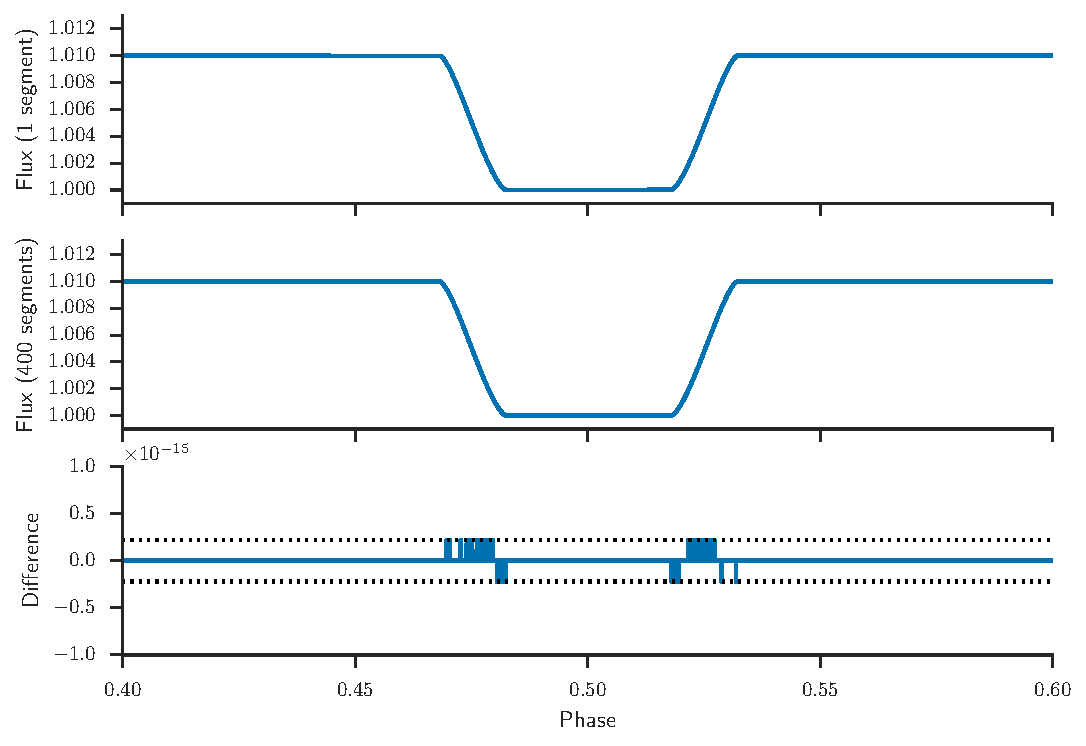
\includegraphics[width=\columnwidth]{img/precision.pdf}
\caption{A comparison between a uniform flux distribution eclipse model generated with 400 segments and a single segment. If the integrator is correct, then there should be no difference between these two models. The bottom panel shows that the results are identical, apart from errors at the level of floating point precision (dotted lines) during ingress and egress.}
\label{fig:precision}
\end{center}
\end{figure}

\subsection{The brightness models}\label{sec:temp model}

\textsc{spiderman} has been written in a modular way, so that users will be able to choose from a variety of models to fit to their data, or provide their own. 

The currently availible models range from fully non-informative to basic physical models, and also utilities to allow the results of forward models to be quickly converted into phase curves and eclipses.

\textsc{spiderman} projects this temperature map onto the visible sphere of the planet, meaning it is used directly to calculate the secondary eclipse and phase curve. 

\subsubsection{Spherical harmonics}

A useful and non-physics dependent model is a sum of spherical harmonics. This method was used for the case of the phase curve of HD\,189733b by \citet{Majeau2012}. An example map generated by \textsc{spiderman} is displayed in figure \ref{fig:harmonics}. The main observational features of a phase curve, including the offset hotspot can typically be recovered with a only the first spherical harmonic, with the centre offset from the substellar point. \citep{Cowan2016} explore the effects of odd harmonics in phase curve data, and find that these correspond to weather features in the planet atmosphere.

\subsubsection{Hotspot models}

The simplest physically model that one construct involve defining a bulk planetary temperature or flux, and then a "Hotspot" where the contrast and offset from the substellar point in longitude and latitude are model parameters. Models where the day and the night side have different fluxes are a subset of these models.

These models could also be used to represent the reflection of light due to clouds in optical phase curves, which have been shown to be present, and even time varying in K2 data \citep{Armstrong2016}.

\subsubsection{Physical model}

\citet{Zhang2016}. This model was developed as part of a simple analytical framework to describe the broad trends within complex GCM's, and does a good job of replicating the temperature distributions of GCM's with only three free parameters. These parameters are physically motivated; the Temperature of the nightside of the planet, $T_n$, the difference in Temperature between the day and night side, $\Delta T$, and the ratio between the advective and radiative timescales in the atmosphere, $\xi$.

The $\xi$ parameter effectively parameterises the degree to which the hotspot of the planet will be offset from the substellar point by the circulation of the plant's atmosphere. The effects of this can be seen in \ref{fig:ex_lcs}, where both the position of the maxima of the phase curve, and the shape of the ingress and egress of the secondary eclipse are clearly effected by this asymmetry.

\begin{figure}
\begin{center}
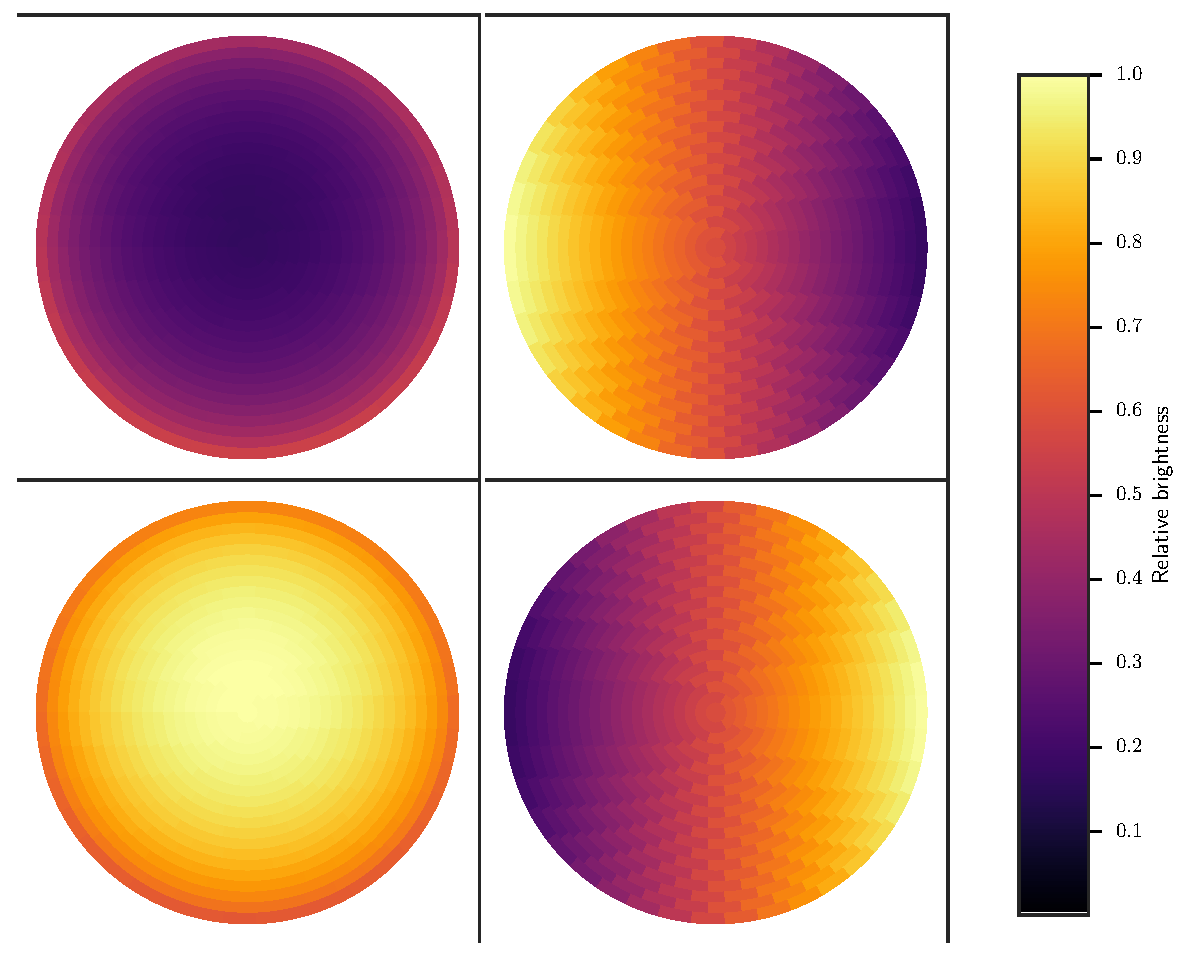
\includegraphics[width=\columnwidth]{img/sphere_quad.pdf}
\caption{A model generated using spherical harmonics}
\label{fig:harmonics}
\end{center}
\end{figure}

\begin{figure}
\begin{center}
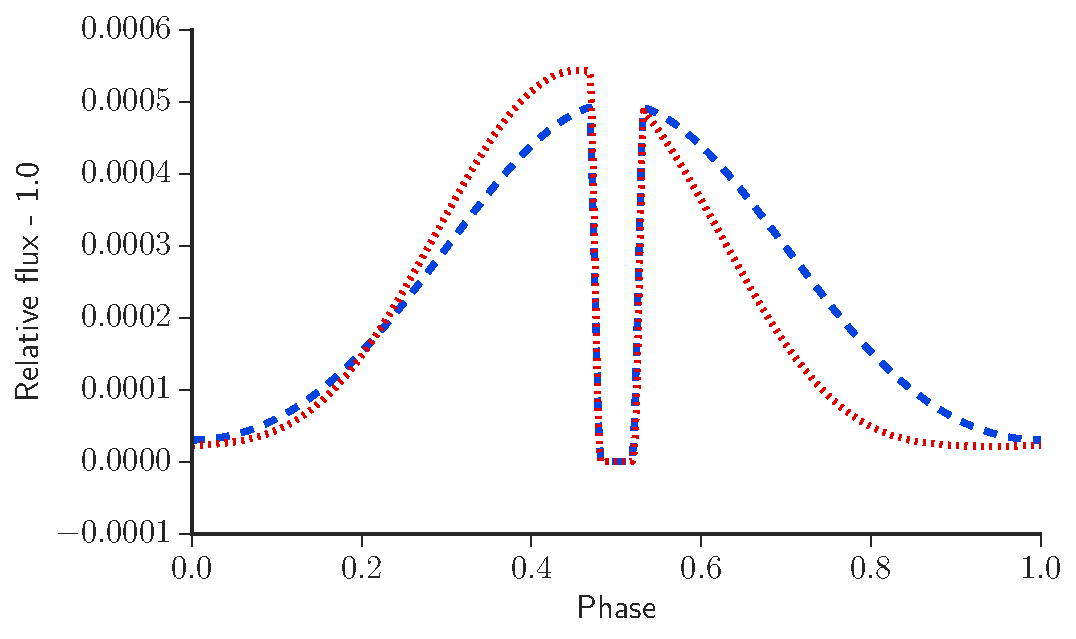
\includegraphics[width=\columnwidth]{img/both_lc.pdf}
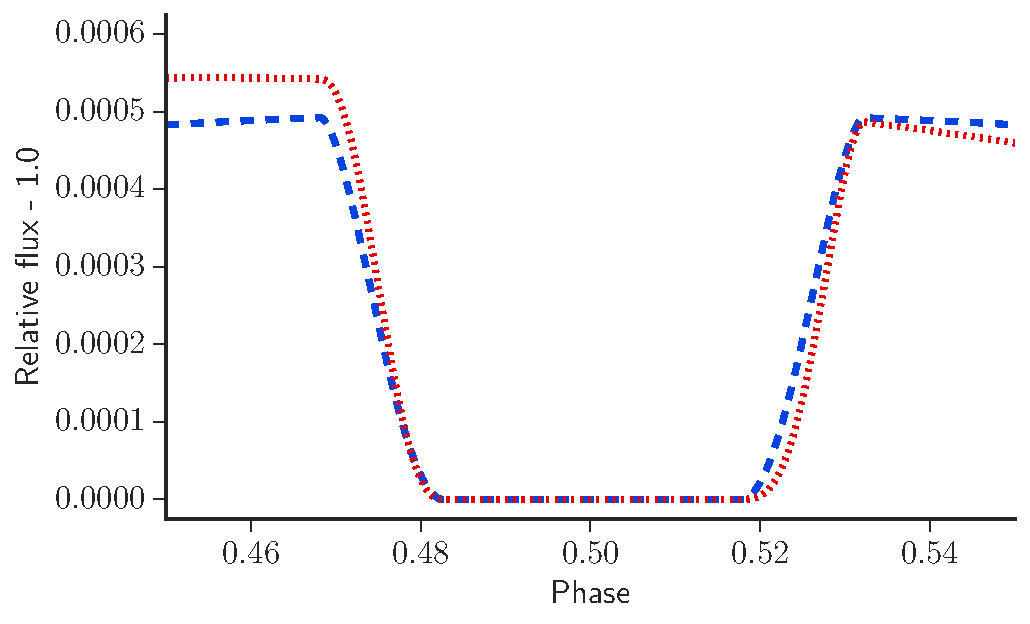
\includegraphics[width=\columnwidth]{img/both_lc_zoom.pdf}
\caption{The phase curve and secondary eclipses of an example planet generated with a simple spherical harmonics flux model (blue dashed) and the \citet{Zhang2016} physical model (red dot). Note in the physical model how the brightest point of the phase curve is significantly offset from the time of secondary transit, and the slightly different shape of the ingress and egress, both caused by the asymmetry in the flux distribution on the planet.}
\label{fig:ex_lcs}
\end{center}
\end{figure}

\subsubsection{Forward model}

\textsc{spiderman} also has the capability to quickly calculate a phase curve and secondary eclipse from a pre-calculated forward model. The code can read in a grid of either temperatures or brightnesses, in longitude and latitude, and will use a two dimensional bicubic interpolation within this grid to assign brightnesses to the grid points at each time-step. Continuity is assumed east-west and across the poles to minimise edge effects.
This is significantly slower than the other models due to the interpolation scheme, but it is assumed that the generation of the forward model is by far the biggest bottle-neck in the calculation, so in this instance speed is not the priority.
This mode is intended to be used in particular for modelling eclipse mapping observations from 3D GCM calculations, either for comparison to data or to test analytical theories.


((figure of 2D GCM results from Viven - would need permission))

\subsubsection{Converting temperature to fluxes}\label{sec:ttof}

Some physical models, such as the one adapted from \citep{Zhang2016}, are defined in terms of temperature, so \textsc{spiderman} must convert that to a flux. To do so we make the assumption that the temperature corresponds to the \emph{brightness temperature} of the planet's photosphere. This will be valid for band passes that are narrower than strong molecular bands in the spectrum, such as water or carbon monoxide, but will not hold over wide band-passes.

There is not an analytical expression for the total amount of flux emitted by a blackbody between two arbitrary wavelengths, so \textsc{spiderman} calculates this value numerically. A grid of blackbody curves multiplied by the instrument response is pre-calculated as a function of temperature, and the flux in the chosen wavelength region is summed numerically. \textsc{spiderman} then linearly interpolates on this grid when assigning fluxes to the planet integration regions based on their temperature.

\subsection{Stellar model}\label{sec:stellar model}

Since the shape and depth of an eclipse and phase curve are determined by the \emph{ratio} of the fluxes between the two bodies, there will clearly be an exact degeneracy between the planet and star brightness. In order to recover physical parameters of the planet, such as temperature, it is necessary to place constraints on the \emph{absolute} scale or brightness of the system. These constraints only need to be on flux as a function of surface area, i.e., on the specific intensity of the system components, and on their radius ratio, not on their total luminosity or radii.

%To see that this is indeed the case, consider a situation where the radii of both the planet and the star have both been underestimated by a factor of 2, but their surface intensities are unchanged, such that the total luminosity will have been underestimated by a factor of 4. The secondary eclipse depth and phase curve amplitude both scale as $(R_p / R_*)^2$, so are unchanged. $(R_p / R_*)^2$ is of course constrained well by the primary transit. The surface brightness distribution as a function of longitude and latitude can therefore be recovered without any constraint on the absolute radii or luminosity of the components.

$(R_p / R_*)^2$ is well constrained from primary transits - the small variation as a function of wavelength is of little importance. There are usually good measurements of the effective temperature of the star from spectroscopy and stellar modelling. These additional parameters fix the flux scale of the system, allowing useful constraints to be placed on the absolute surface flux and brightness temperature of the planet.

\textsc{spiderman} models the stellar spectrum using a grid of PHOENIX stellar atmospheres calculated by \citet{Husser2013}. Using the user provided wavelength bandpass and instrument response, \textsc{spiderman} calculates the total observed flux for the available models as a function of effective temperature, it then interpolates on this grid using a spline.

\subsection{Lightcurve calculation}\label{sec:lightcurve}

The primary purpose of \textsc{spiderman} is to produce lightcurves to compare with the data. Now that the functioning of the geometric integrator has been described, lightcurve generation is quite simple.

Given a series of time points, the ephemeris of the system, the system scale and the planet star radius ratio, the position of the planet relative to the star can be calculated for each timestep. Light time of travel effects are accounted for, with the semi-major axis in physical units as a parameter.

Since it is assumed that the planet is tidally locked, at each timestep the geometric grid representing the planet is populated with the appropriate fluxes from the chosen flux distribution model.

Then, for each segment on the planet, it is checked whether it is currently being occulted. This is quickly achieved by checking for contact between the edges of the region and the edge of the star. If there are no contact points, and the distance from the center point to the center point of the star is greater than the stellar radius, then the segment is fully visible, and the full flux is counted, if the distance is less then the stellar radius then it is fully occulted and no flux is added. For cases of partial coverage, the previously described geometric integrator is used to calculate the flux that should be added.

To this, the pre-calculated stellar total flux is added to give the total system flux. This is then divided by the stellar flux to give a relative lightcurve that can easily be compared to data.

Note that \textsc{spiderman} does not calculate primary transits. To fit models to data that contain both primary and secondary eclipses, \textsc{spiderman} should be combined with another package such as BATMAN. The parameter naming convention and call sequence from \textsc{spiderman} has been chosen to be compatible with BATMAN for this reason. 

\section{The \textsc{spiderman} package}\label{sec:package}

\textsc{spiderman} is an open source project and is being actively developed on github. The code is available on PyPi and github at \url{https://github.com/tomlouden/spiderman}.

%\begin{Verbatim}[frame=single]
%> pip install spiderman-package
%\end{Verbatim}

%Or, to access the development version from github:

%\begin{Verbatim}[frame=single]
%> git clone https://github.com/tomlouden/SPIDERMAN
%> cd SPIDERMAN
%> sudo python setup.py install
%\end{Verbatim}

Installation instructions and documentation are available at \url{http://spiderman.readthedocs.io}

%A model instance is initialised by typing

%\begin{Verbatim}[frame=single]
%> spider_params = spiderman.ModelParams(MODEL)
%\end{Verbatim}

%Where MODEL is the chosen surface brightness distribution. The model parameters are then entered, and from there, generating a lightcurve to compare to data is as simple as entering

%\begin{Verbatim}[frame=single]
%> spider_params.lightcurve(t)
%\end{Verbatim}

%Where t an array of timepoints where the model is to be evaluated.

%\textsc{spiderman} comes prepackaged with several plotting scripts to make visualisation of the model simple.

%Typing the command

%\begin{Verbatim}[frame=single]
%> spider_params.plot_planet(t)
%\end{Verbatim}

%\begin{Verbatim}[frame=single]
%> spider_params.plot_system(t)
%\end{Verbatim}

As well as lightcurve generation the code includes plotting functions to visualise the brightness or temperature distributions. An example plot is given in \ref{fig:plot_system}, which is a scale diagram of the system at a specified time or phase. Plots like this are useful for visualising the effects of varying the parameters.

\begin{figure*}
\begin{center}
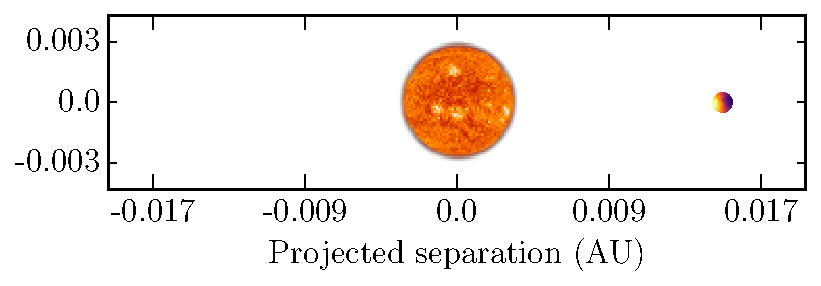
\includegraphics[width=\textwidth]{img/system.pdf}
\caption{An example of the graphical output that \textsc{spiderman} can produce. This image is a scale representation of the system, with the planetary flux map included. This is useful for visualising the model. It was generated with the spiderman.plot\_system() command. The image of the star is purely aesthetic.}
\label{fig:plot_system}
\end{center}
\end{figure*}

In typical usage, SPIDERMAN is capable of producing over 1000 models per second on a single core. This means that a 1 million MCMC sample can be generated in approximately a quarter of an hour.

Figure \ref{fig:exec_time} shows the result of a performance test carried out on a single core of an Intel Core I5-3470 Processor. The length of time to produce a model with 1000 timepoints as a function of the number of segments of the model. The test shows that the execution time scales linearly with the number of segments in the model, which is expected, showing the overhead to run the model is very small. The precision required for typical usage can easily be reached using 16 or 25 segments, but larger numbers of segments can be used to produce better looking diagrams. The diagrams in this paper were generated with a 400 segment model.

\begin{figure}
\begin{center}
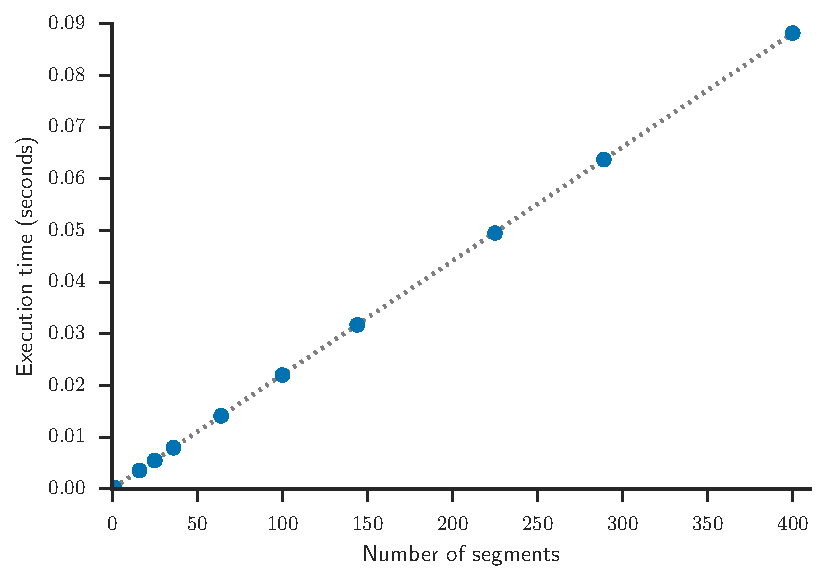
\includegraphics[width=\columnwidth]{img/exec_time.pdf}
\caption{The speed with which a model with 1000 timepoints can be generated}
\label{fig:exec_time}
\end{center}
\end{figure}

\section{Application to data}\label{sec:Application}

As a test of the performance of the code the model was applied to a phase curve and secondary eclipse of WASP-43b taken with HST WFC3. These data have previously been published in \citet{Stevenson2014}. However, in their paper the phase curve is fit with a sinusoid function. Here we instead apply the physically motivated model of \citet{Zhang2016} to test its applicability to observed data. This also reduces the total number of parameters needed for the fit.

Planetary Limb darkening is a potential sources of uncertainty on the final brightness distribution that would require more detailed atmosphere models to predict. \textsc{spiderman} has the option to include planetary limb darkening in addition to the chosen brightness model with a quadratic law. In principle, measurements of planetary limb darkening can constrain the vertical temperature profile of the planet, however this would require a full radiative transfer treatment calculation of the atmosphere. For the case of WASP-43b, limb darkening is not expected to be important, since the planet appears to have a near isothermal profile \citep{Stevenson2014}, which should correspond to zero limb darkening. We treat the additional freedom from the limb darkening as a test of the sensitivity to uncertainties of the radial brightness profile of the planet.


\subsection{Systematics model}\label{sec:systematics}

As with most exoplanet observations with Hubble, the data are effected by the idiosyncratic systematic errors of the instrument. Fortunately, the sources of these errors are relatively well understood, and are generally quite repeatable between observations. They are therefore quite straightforward to fit for and remove. 

The systematics have effects on scales of \emph{visits}, \emph{orbits} and individual exposures, where a visit is a continuous set of orbits directed at a target. Due to the low earth orbit of Hubble, each complete orbit lasts 95 minutes, and for approximately half of this time the target will be unobservable due to being behind the Earth. For this reason, a complete exoplanet transit can not be observed with one ``visit", and it is necessary to observe several transits with different temporal phasing to completely cover the full orbital phase of the system.

In this study, three visits, each with 12 orbits was used to cover the full phase of WASP-43. The phasing can be seen in figure \ref{fig:systematics}, and a phase folded lightcurve can be seen in figure \ref{fig:phase folded}

The systematics model we use to fit WASP-43 is the same that was used in the previous treatment \citep{Stevenson2014}. There are three components to the systematics model, the scan direction offset, ``hook effect'' and visit long slopes.

The scan direction offset is depends on which way the the ccd was scanning during the readout, in one half of exposures the scan direction is in the same direction as the readout, and in the other half it is the offset. This leads to a very repeatable offset in the fluxes between the two scan directions, which can be captured with a single parameter \emph{scale}

Each orbit displays a characteristic exoplential ``hook'' signal, which can be modelled as
\begin{equation} \label{eq:hook}
F_{cor} = F*(1-exp(-r1 t_{orb}-r2-r3 \delta_{fo}))
\end{equation}
Where $F$ is the flux before correction and $F_{cor}$ is the corrected flux $t_{orb}$ is the time from the start of each \emph{obit}, $r1$, $r2$, $r3$ are the fitted coefficients. This exponential ramp has a different shape during the first orbit of a visit, so the $\delta_{fo}$ function takes a value of 1 if the orbit is the first, and 0 at all other times. The exponential hook shape is believed to be related to charge trapping, and is a characteristic and repeatable feature across orbits, so these parameters are fit simultaneously over visits.

Each \emph{visit} displays a decreasing slope, which is modelled as a second order polynomial. The cause of these features is unknown, and they have not been linked to any physical parameters of the telescope \cite{Wakeford2016}. Here, they are also likely blended with the ``Breathing" systematics of the instrument, which are caused by the changing thermal environment of the telescope during its orbit changing the focal length of the instrument. The shape of these visit long effects is slightly different between the three visits used here, so the three paramters of the polynomial are fit seperately for the three visits.

The feature that is the greatest cause for concern is the visit long slope in the data, as this has a comparable timescale and amplitude to the planet's phase curve, so there is potential for degeneracies between the systematics and physical models.

Fortunately, the phasing of the observations is such that the three visits cover different portions of the phase curve, which helps to alleviate the degeneracy.

For HST systematics, where the major sources of error are fairly well understood, a parametrised systematics model of this form works well \citet{Wakeford2016}. Alternatively, detailed instrumental models can recover the same features with fewer free parameters, however if the form of the systematics changes over time then this approach might underestimate the uncertainty in the shape of the systematics and thus artificially constrain the planet models.

An alternative, powerful technique which does not make assumptions about the form of the systematics is Gaussian Processes \citep[e.g.][]{Gibson2012a}. ((Find a more recent reference with regards to JWST, or the one comparing sytematis models on HST and spitzer))
%Future analysis of this dataset could use a Gaussian process noise model instead of the parametrised one featured here, as used in \citet{Gibson2012a}, this could provide further confidence in the results, as the added flexibility of the GP model and the explicit fit for the timescale of the features would allow the degeneracy to be explored with fewer explicit hyper-parameters.

An important early result from JWST will be a characterization of the systematics, particularly for MIRI, as this will have significant consequences for the practicality of phase curve and eclipse mapping observations with JWST.

\subsection{MCMC}\label{sec:MCMC}

In order to properly access the errors on the parameter values of interest, and test for degeneracies with the systematics model, we perform an MCMC analysis. We use the \textsc{emcee} affine invariant Monte Carlo implementation of \citet{Foreman-Mackey2013}.

The initial parameter positions are found with a least squares minimization approach, and the 1000 walkers were initialized around these best fitting values.

For the orbital and system parameters we use published values and errorbars as priors. For the Period, inclination and $a/R_*$ we use the results of \citet{Hoyer2016}, and for $a$ the value from \citet{Hellier2011a}, The eccentricity was fixed at 0, which is supported by the findings of \citet{Hoyer2016}. The stellar log g and effective temperature priors are from \citet{Gillon2012}.

To test for the potential impact of \emph{planetary} limb darkening, we ran a separate MCMC with this effect modeled by a simple quadratic limb darking law with parameters $p_{u1}$ and $p_{u2}$. We place the constraint that the limb darkening must be monotonic across the disc of the planet, i.e., there can be no change in the sign of the gradient. This results in profiles that are either flat, wholly limb darkened or wholly limb brightened, with no overly flexible profiles.

For both models, the MCMC was run for 10 million steps, with the first 200,000 steps discarded as burn in.

\subsection{Results and discussion}\label{sec:results}

The best fitting model and the residuals are shown in figure \ref{fig:phase folded} as a function of planetary phase, after correction for instrument systematics. The data and model are also plotted as a function of time in figure \ref{fig:systematics}. To demonstrate the systematics model the data are plotted with and without systematics correction.

\begin{figure}
\begin{center}
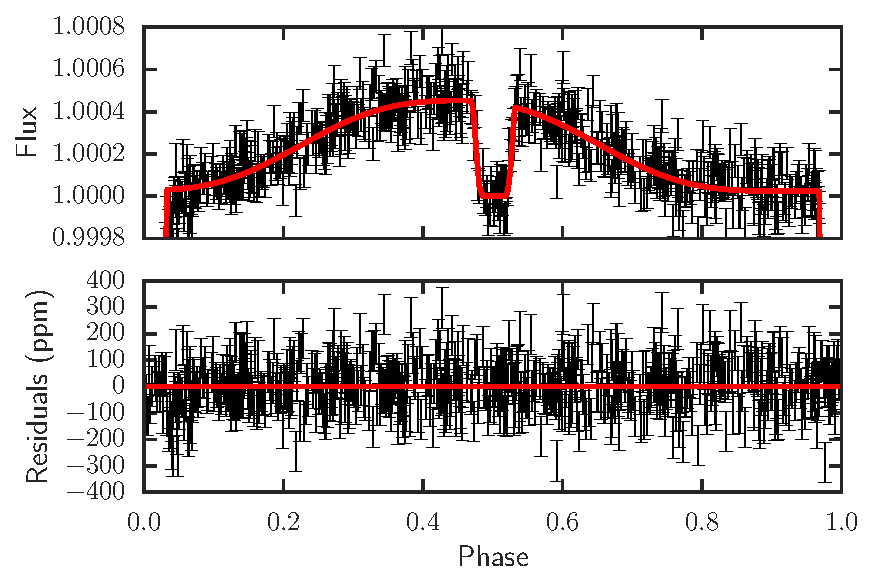
\includegraphics[width=\columnwidth]{img/new_lc.pdf}
\caption{The final fitted lightcurve. The primary transit is fit by \textsc{batman} and is off the scale of this figure.}
\label{fig:phase folded}
\end{center}
\end{figure}

The results of both runs are presented In table \ref{tab:results}. With the exception of $T_n$, which is lower by more than $3\sigma$ in the fit with planetary limb darkening, the physical parameters are consistent. In particular, $\xi$ seems only weakly affected by the presence of limb darkening, the difference being much less than $1\sigma$. This is not unexpected, as $\xi$ effectively parametrises the asymmetry in the flux distribution, while the limb darkening is symmetrical. $\xi$ is directly tied to the details of heat transport in the atmosphere, so the insensitivity of this parameter to limb darkening is useful, as it shows that it can be recovered even with systematic uncertainties in the flux distribution, so long as they are symmetric.

\begin{figure}
\begin{center}
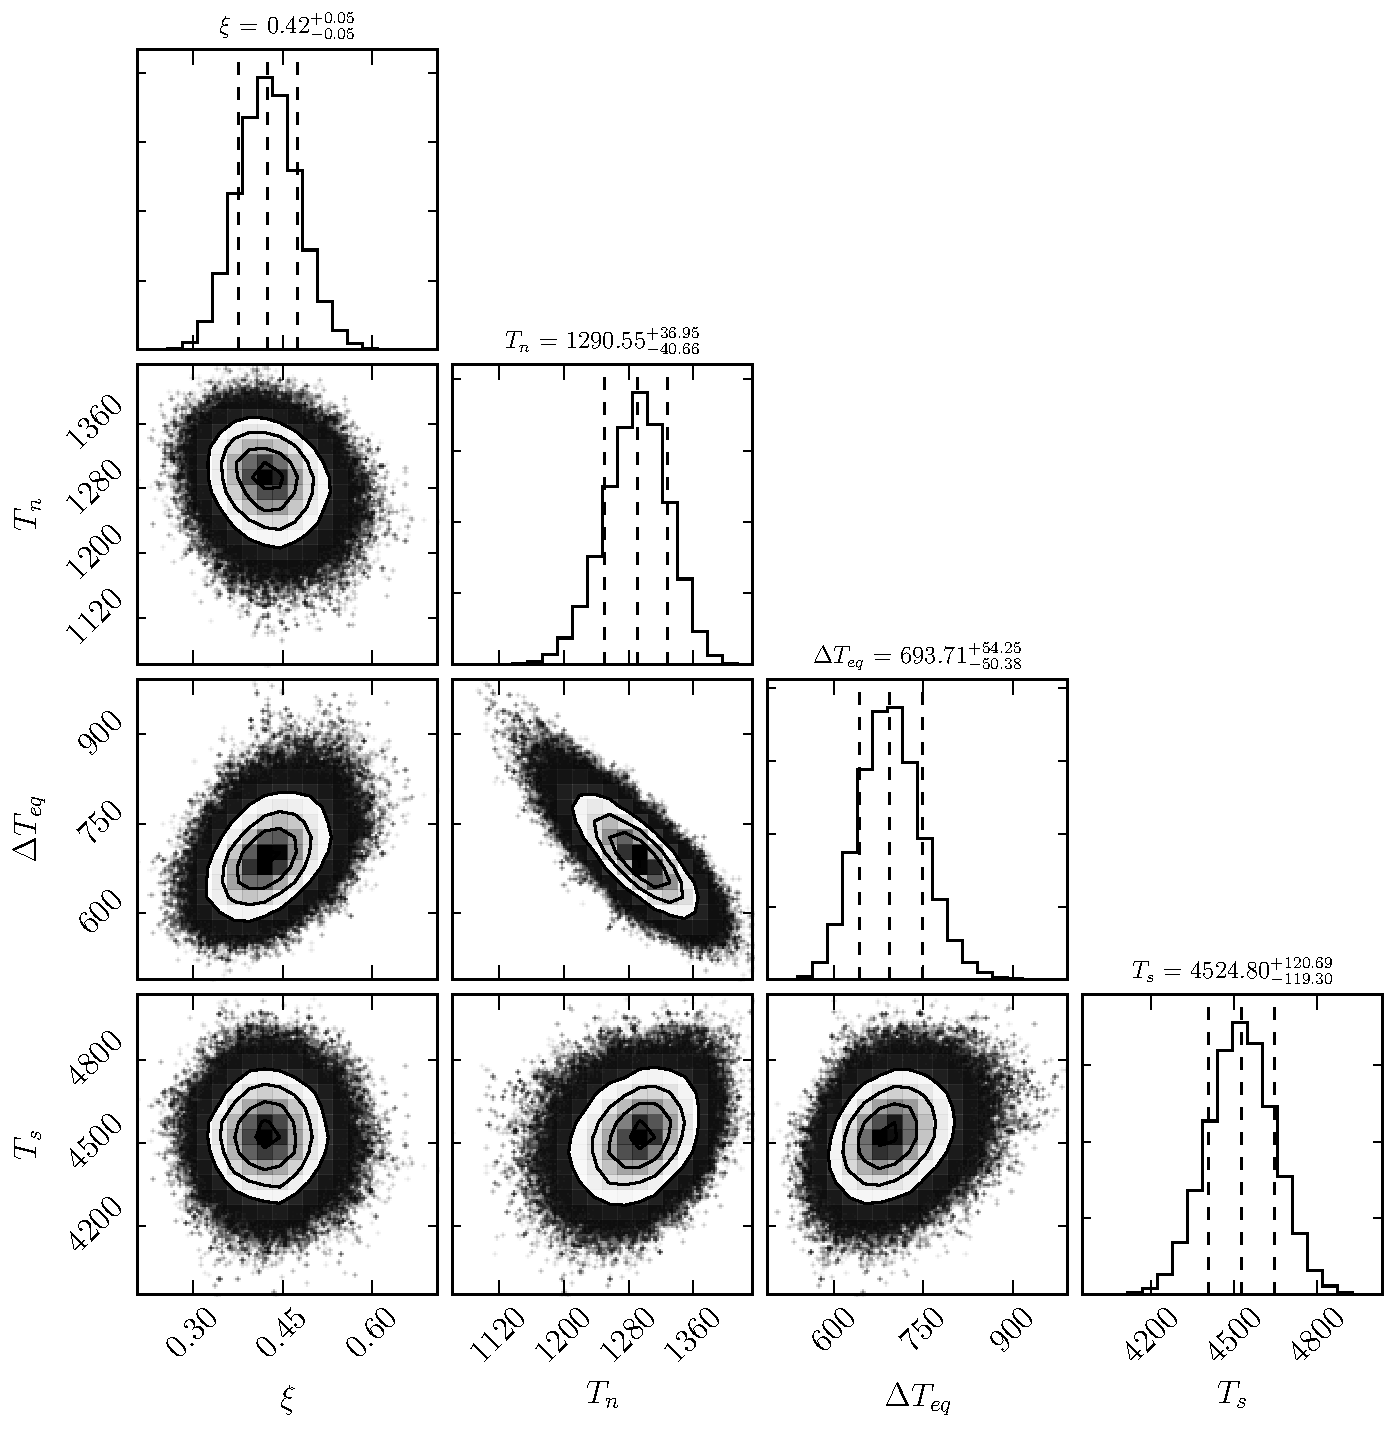
\includegraphics[width=\columnwidth]{img/free_parameterstriangle.pdf}
\caption{A section of the corner plot focusing on the key model parameters. The parameters for the Zhang model fit are loosely correlated. The distribution for the stellar temperature, $T_s$, is set by the prior}
\label{fig:triangle corner sub}
\end{center}
\end{figure}

The correlation between the physical model with the other model parameters can be seen in figure \ref{fig:triangle corner sub}. $T_s$ and $\Delta T$ are clearly correlated parameters, since between them they determine the average temperature of the dayside and hence the amplitude of the phase curve. $\xi$ is not strongly degenerate with the other parameters. This indicates that the $\xi$ parameter is robust to any errors in the absolute flux level of the system.

The visual representation of the flux maps for the non-limb darkened case can be seen in figure \ref{fig:best_fit_flux}. The best fitting model is displayed at 4 phases, as well as the relative error on the flux distribution. The error map was generated by drawing 10,000 maps from the MCMC posterior and taking the standard deviation of the fluxes in each segment. The offset hot-spot is significant and clearly visible. The underlying temperature maps, and the errors in these, are shown in figure \ref{fig:best_fit_temp}.

The model fit implies that the night-side of the planet is significantly hotter than expected at 1290 $\pm 39$ K, whereas it is not significantly detected in \citet{Stevenson2014}. If the nightside has been detected, the flux immediately before and after primary transit should be significantly different to the star-only flux visible during the secondary eclipse. Drawing 10,000 lightcurves from the parameters in the non-limb darkened MCMC posterior, we plot the median, 1 sigma and 3 sigma contours for the lightcurve in figure \ref{fig:model}. The flux is found to be greater than 1.0 at the 3 sigma level.

\begin{figure}
\begin{center}
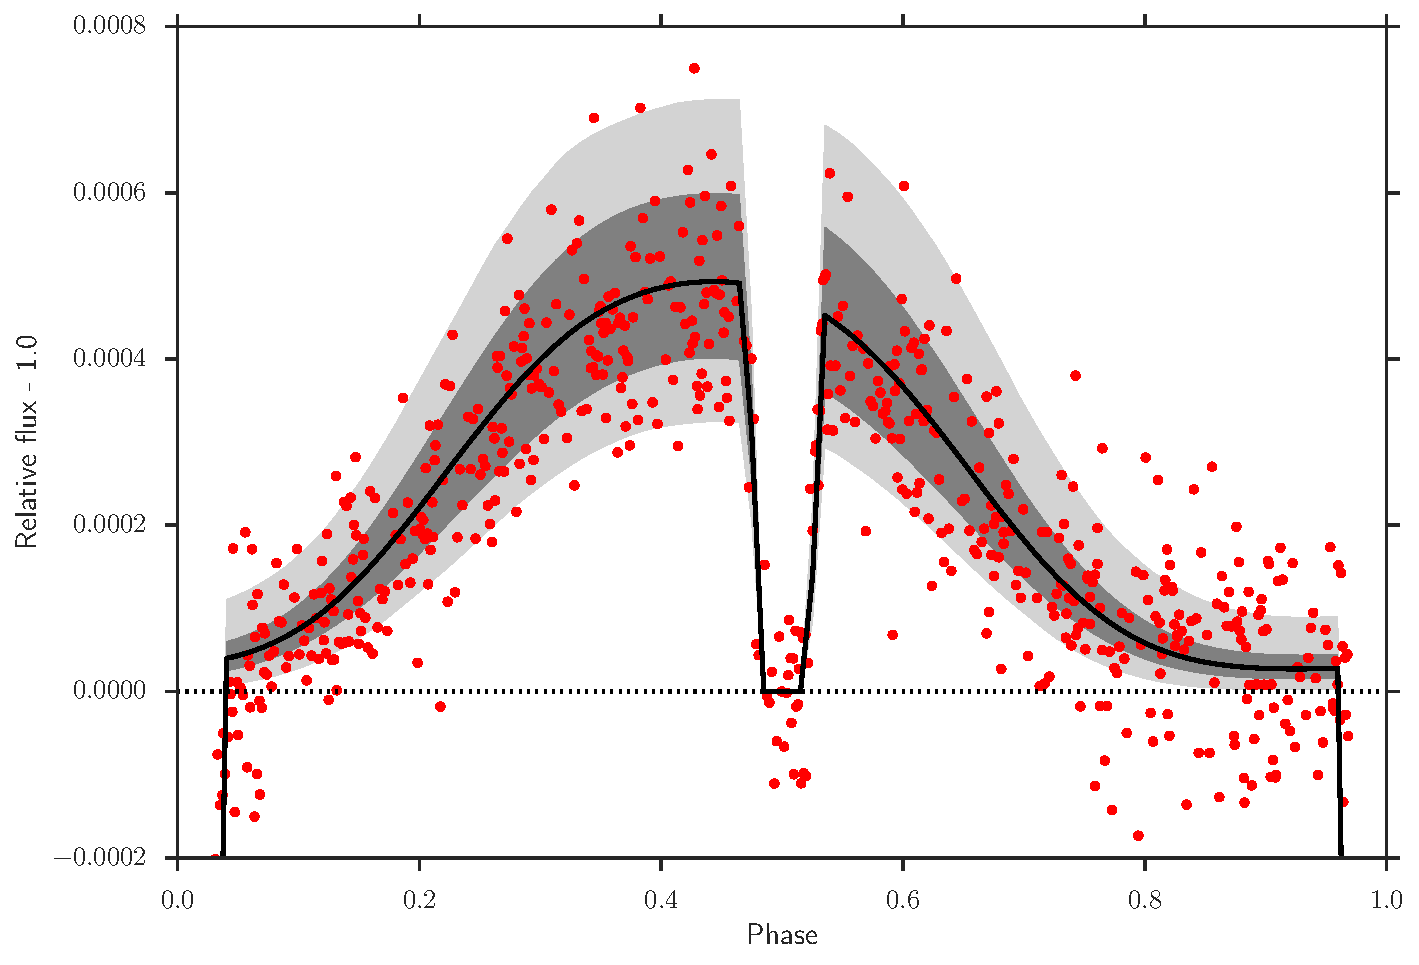
\includegraphics[width=\columnwidth]{img/model.pdf}
\caption{the uncertainty on the model from the MCMC fit. There is a greater than 3 sigma detection of night-side flux.}
\label{fig:model}
\end{center}
\end{figure}

%((Laura - comment on how bright nightside would be inconsistent with eclipse spectra?))

The fit with limb darkening finds a significantly fainter night side flux, suggesting that the nightside flux is an artifact of using a simple physical model. This may be due to a correlation between model parameters making the fit inflexible and the simultaneous fit with the systematics model. Alternatively, the model may be unable to parametrise a feature of the nightside that is blocking the emitted flux, such as clouds.

However, we emphasize that the $\xi$ parameter does not seem to be effected, which raises our confidence in the robustness of the fit to any potential errors in the symmetric radial component of the surface map.

%\begin{figure}
%\begin{center}
%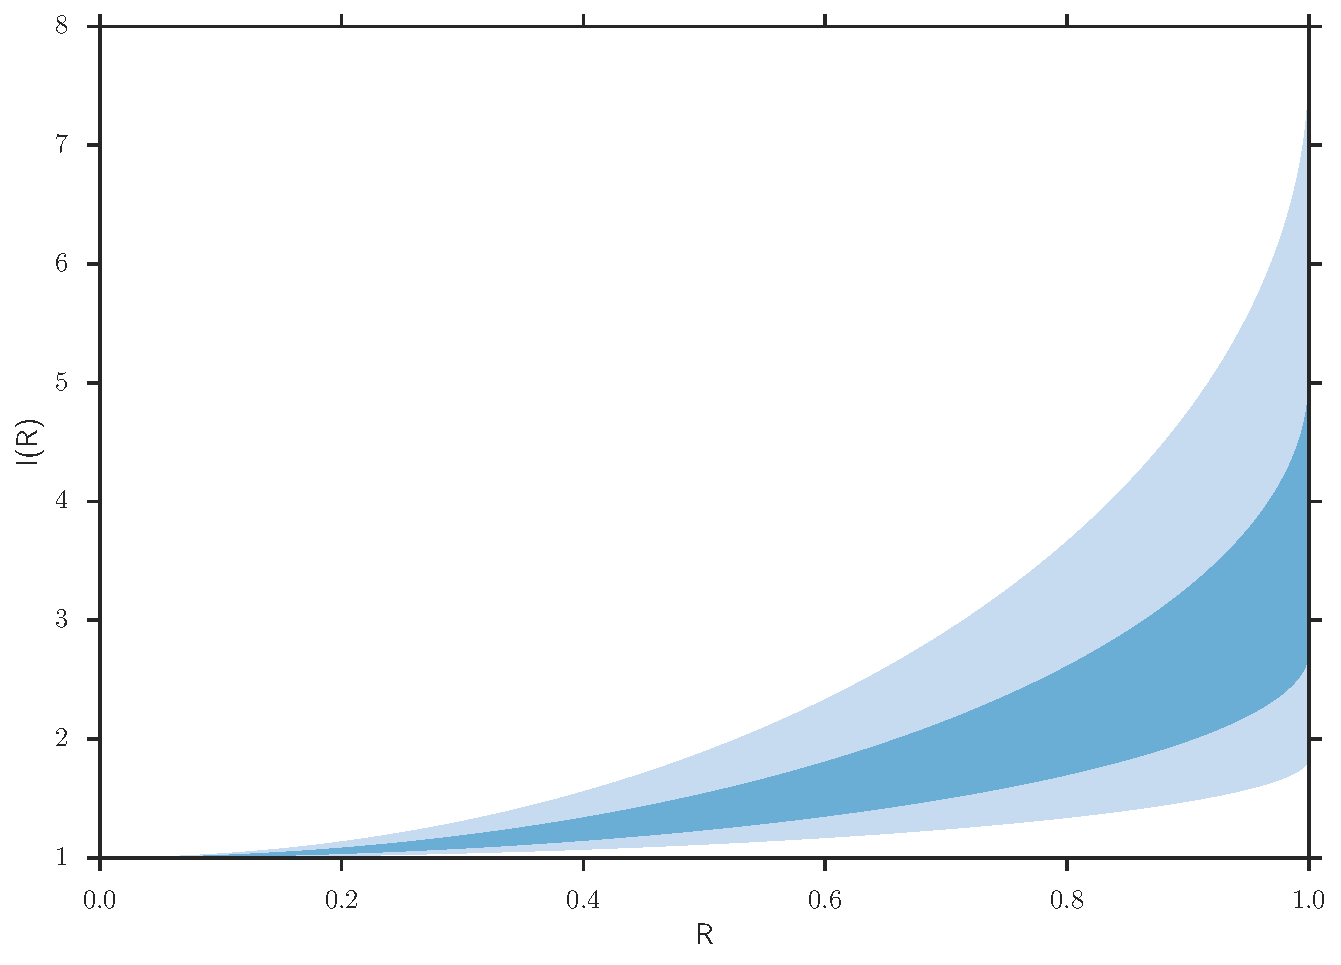
\includegraphics[width=\columnwidth]{img/ld_prof.pdf}
%\caption{The 1 sigma and 3 sigma contours for the Radial intensity profile of the planet, indicating that the fit has a significant preference for limb brightened profiles }
%\label{fig:limb brighten}
%\end{center}
%\end{figure}

\begin{center}
\begin{table*}{
\caption{The full results from the MCMC fit both with and without planetary limb darkening included.}
\begin{center}
\begin{tabular}{l c c c c c}
\hline
\hline
          &   ld fixed   &             &   ld free    &             \\
name      &   median     & error       &   median     & error        & unit        \\
\hline
Period &  0.813473977 & $\pm$ 0.000000036 &  0.813473979 & $\pm$ 0.000000034 & days\\
$t0$ & 2456601.0274024 & $\pm$   0.0000091 & 2456601.0274025 & $\pm$   0.0000091 & days\\
$a/R_*$ &       4.8762 & $\pm$      0.0089 &       4.8772 & $\pm$      0.0087 & -\\
inclination &       82.123 & $\pm$       0.038 &       82.125 & $\pm$       0.037 & degrees\\
eccentricity & 0 & - & 0 & - & -\\
$R_p/R_*$ &     0.159692 & $\pm$    0.000093 &     0.159650 & $\pm$    0.000092 & -\\
$u1$ &       0.3880 & $\pm$      0.0083 &       0.3875 & $\pm$      0.0082 & -\\
$u2$ & 0 & - & 0 & - & -\\
$c_1$ & 3.687319e+08 & $\pm$    0.000090e+08 & 3.687526e+08 & $\pm$    0.000089e+08 & -\\
$c_2$ & 3.693661e+08 & $\pm$    0.000097e+08 & 3.693654e+08 & $\pm$    0.000097e+08 & -\\
$c_3$ & 3.689717e+08 & $\pm$    0.000093e+08 &  3.68984e+08 & $\pm$     0.00010e+08 & -\\
$v1_1$ &   -1.484e+06 & $\pm$       0.045e+06 &   -1.559e+06 & $\pm$       0.049e+06 & -\\
$v1_2$ &    -6.31e+05 & $\pm$        0.50e+05 &    -6.19e+05 & $\pm$        0.55e+05 & -\\
$v1_3$ &    -8.56e+05 & $\pm$        0.49e+05 &    -8.57e+05 & $\pm$        0.54e+05 & -\\
$v2_1$ &    1.004e+06 & $\pm$       0.059e+06 &    1.076e+06 & $\pm$       0.064e+06 & -\\
$v2_2$ &     1.83e+05 & $\pm$        0.61e+05 &     1.92e+05 & $\pm$        0.67e+05 & -\\
$v2_3$ &     4.08e+05 & $\pm$        0.62e+05 &     3.77e+05 & $\pm$        0.67e+05 & -\\
$r1$ &        123.2 & $\pm$         3.5 &        122.7 & $\pm$         3.5 & -\\
$r2$ &        5.874 & $\pm$       0.011 &        5.877 & $\pm$       0.011 & -\\
$r3$ &       -0.087 & $\pm$       0.028 &       -0.113 & $\pm$       0.028 & -\\
scale &   -0.0024748 & $\pm$   0.0000061 &   -0.0024749 & $\pm$   0.0000060 & -\\
$p_{u1}$ & 0 & - &         -1.2 & $\pm$         0.9 & -\\
$p_{u2}$ & 0 & - &         -2.7 & $\pm$         1.1 & -\\
$a$ &      0.01421 & $\pm$     0.00040 &      0.01419 & $\pm$     0.00040 & AU\\
$\xi$ &        0.436 & $\pm$       0.050 &        0.417 & $\pm$       0.053 & -\\
$T_n$ &         1290 & $\pm$          39 &         1069 & $\pm$          62 & K\\
$\Delta_T$ &          699 & $\pm$          53 &          827 & $\pm$          92 & K\\
$T_s$ &         4530 & $\pm$         120 &         4530 & $\pm$         120 & K\\
\end{tabular}
\end{center}
\label{tab:results}
}
\end{table*}
\end{center}

\subsubsection{Spectrally resolved}

Spectrally resolving the phase offset in principle allows information on the heat transport as a function of depth. To test for this effect we break the data down into 15 spectral bins and repeat the MCMC analysis described for the white light data, without allowing the additional radial freedom from limb darkening. We fix the system parameters to those found in the white light fight. We report the measurement of $\xi$ parameter as a function of wavelength in table

\begin{table}{
			\caption{Fits to the spectrally resolved data}
			\begin{center}
				\begin{tabular}{c c}
					\hline
					\hline
					Central wavelength &   log10(xi)  \\
					(microns) & \\
					\hline
1.1425 & -0.32 $\pm$ 0.27 \\
1.1775 & -0.51 $\pm$ 0.32 \\
1.2125 & -0.00 $\pm$ 0.18 \\
1.2475 & -0.20 $\pm$ 0.19 \\
1.2825 & -0.74 $\pm$ 0.39 \\
1.3175 & -0.32 $\pm$ 0.19 \\
1.3525 & -0.82 $\pm$ 0.62 \\
1.3875 & -0.07 $\pm$ 0.20 \\
1.4225 & -0.09 $\pm$ 0.34 \\
1.4575 & -0.71 $\pm$ 0.31 \\
1.4925 & -0.42 $\pm$ 0.17 \\
1.5275 & -0.76 $\pm$ 0.37 \\
1.5625 & -0.43 $\pm$ 0.14 \\
1.5975 & -0.66 $\pm$ 0.25 \\
1.6325 & -0.59 $\pm$ 0.19 \\
\end{tabular}
\end{center}
\label{tab:specresults}
}
\end{table}

\begin{figure}
	\begin{center}
		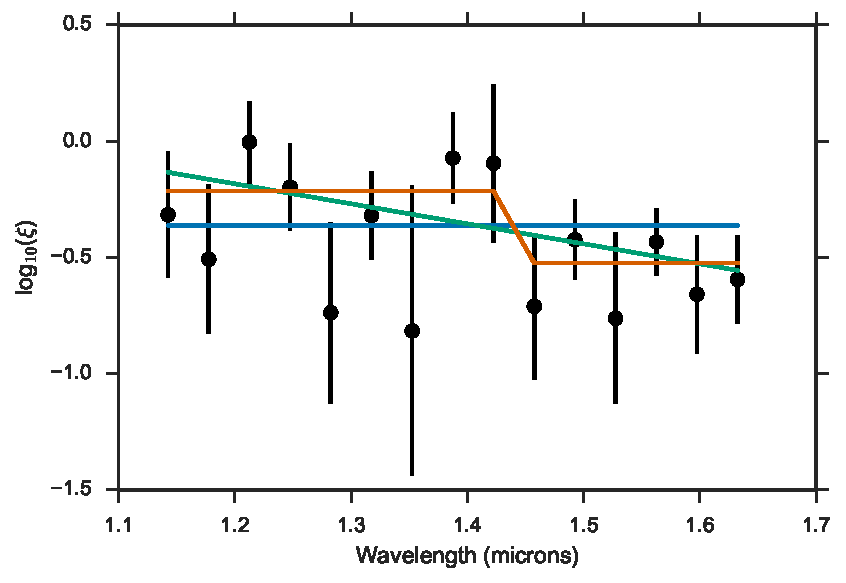
\includegraphics[width=\columnwidth]{img/all_models.pdf}
		\caption{This alright fit to Xi as a function of wavelength. blue: flat line, green: gradient function, orange: step function}
		\label{fig:best_fit_flux}
	\end{center}
\end{figure}

The flat model gave a value of -0.36 - note that this is a good match to the white light value. This gave an acceptable fit, with a chi2 of 15.1 (R chi2 of 1.16) with 14 DOF

The best fitting gradient model had values -0.8606214   0.84938152 and gave a chi2 of 8.8 (RCHI2 0.67) with 13 DOF

The best fitting model was the step function model with a dividing wavelength of 1.4225 microns, and step values of -0.5242412 -0.2149221. This gave a chi2 of 8.0 (R chi2 of 0.62) with 12 DOF.

While we find that there is weak evidence for a trend with wavelength in the data, the flat line model provides a satisfactory fit to the data.

\section{Conclusions}\label{sec:conclusions}

In this paper we have introduced \textsc{spiderman}, an open source code for modelling phase curves and secondary eclipses with arbitrary brightness distributions. The code is modular and able to use a variety of different brightness distributions.

The C based algorithm analytically calculates the area occulted of radial segments on the planet's surface, and is designed to run rapidly to enable statistical techniques such as MCMCs to run quickly.

We demonstrate the use of \textsc{spiderman} by applying the code to the case of WASP-43b. We use a physically motivated analytical model presented by \citet{Zhang2016} which captures the major features of exoplanet phase curves. We find that the model provides a good fit to the data, but overpredicts the nightside flux compared to non-informative models. We hypothesise that this may be due to the presence of clouds on the planet's nightside.

As the exoplanet community prepares for a wealth of high precision phase curves and eclipses from new facilities such as TESS and JWST, we release \textsc{spiderman} as an easy to use software package that will enable robust analysis of these high precision data.

%\section{Future work}\label{sec:future work}

%\textsc{spiderman} is still under development, and there are a number of features that are planned to be implemented:

%\begin{itemize}
%\item More thermal brightness distributions, such as an ``orange segments'' model and a simple parametrised hotspot which can be offset in latitude and longitude
%\item Implement \emph{reflected} light phase curves and secondary eclipses, through adding appropriate brightness distributions like Lambertian reflectors and patchy clouds.
%\item Allow calculation of multiple spectral channels simultaneously, with linked system parameters.
%\item Include instrument response in calculating flux ratios
%\item Better treatment of errors in the spectral energy distribution of the star - include errors in log-g and Metalicity
%\end{itemize}

%In regards to the re-analysis of WASP-43bs phase curve, future analysis will focus on:

%\begin{itemize}
%\item Confirming the detected flux on the nightside is a real feature and not an artefact
%\item Further test for degeneracies between HST systematics and the physical model of the phase curve, in particular the combination of visit long slope and breathing modes. This could be accomplished by a Gaussian process analysis.
%\item Perform recovery with a non-informative model, such as spherical harmonics, and see if the recovered brightness or temperature maps are the same as recovered through physical models.
%\item Investigating the apparent preference for limb brightened profiles in the model fit. This is characteristic of a temperature inversion, but since there is no evidence for this in other data on WASP-43b it may be more likely that it indicates a weakness of the model.
%\item Making wavelength resolved maps. This will allow spectra as a function of latitude and longitude to be created. The wavelength also functions as a proxy for height in a planetary atmosphere, so the map will effectively be three dimensional.
%\item Investigate correlations between spectrally resolved bins and consider the impact of simultaneous fits.
%\end{itemize}

\begin{figure*}
\begin{center}
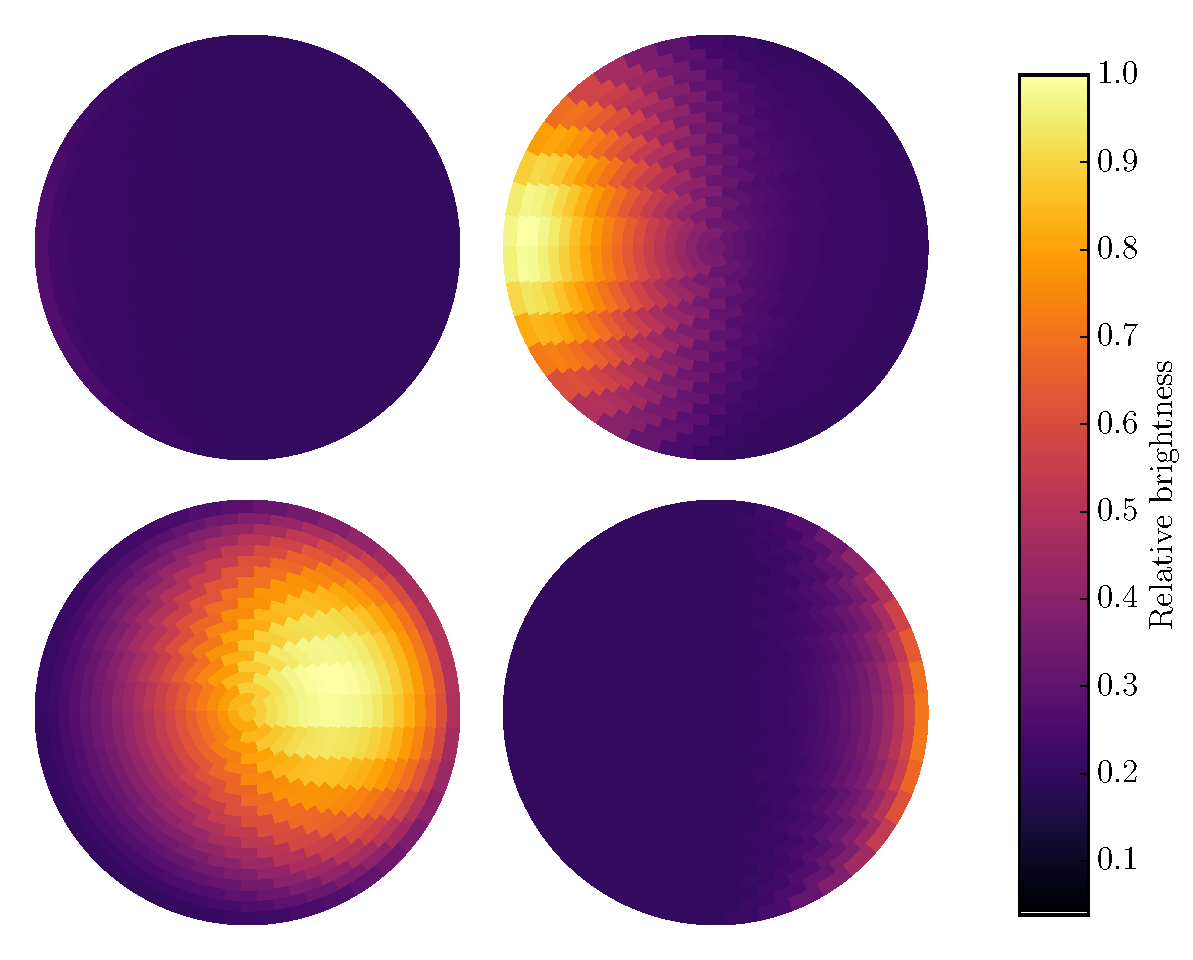
\includegraphics[width=\columnwidth]{img/free_parametersflux_map.pdf}
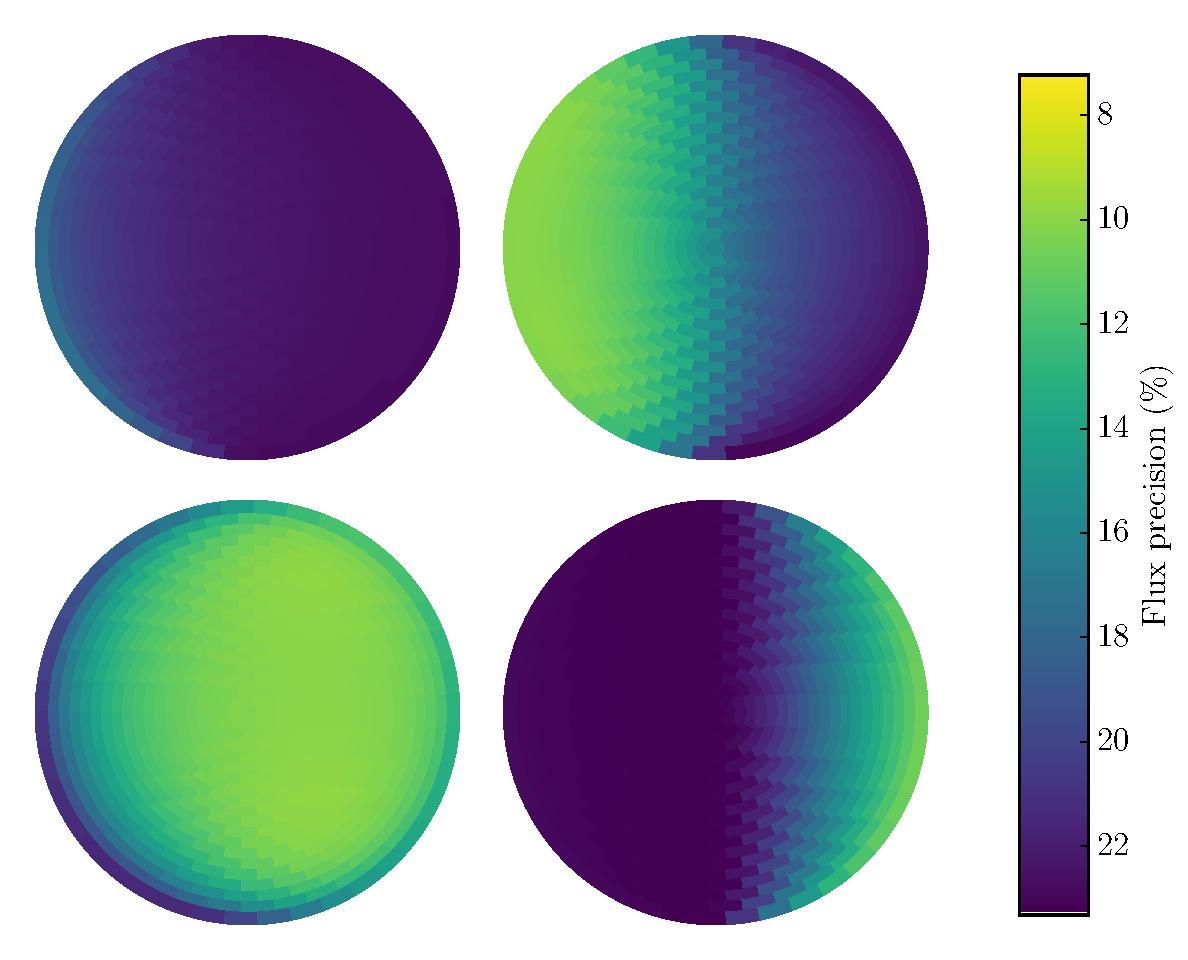
\includegraphics[width=\columnwidth]{img/free_parametersflux_errs.pdf}
\caption{left: The best fitting flux distribution for the model where the planetary limb darkening was switched off at 4 phases, from top left clockwise the phases are 0, 0.25, 0.75 and 0.5. right: The respective constraints on the brightness distribution}
\label{fig:best_fit_flux}
\end{center}
\end{figure*}

\begin{figure*}
\begin{center}
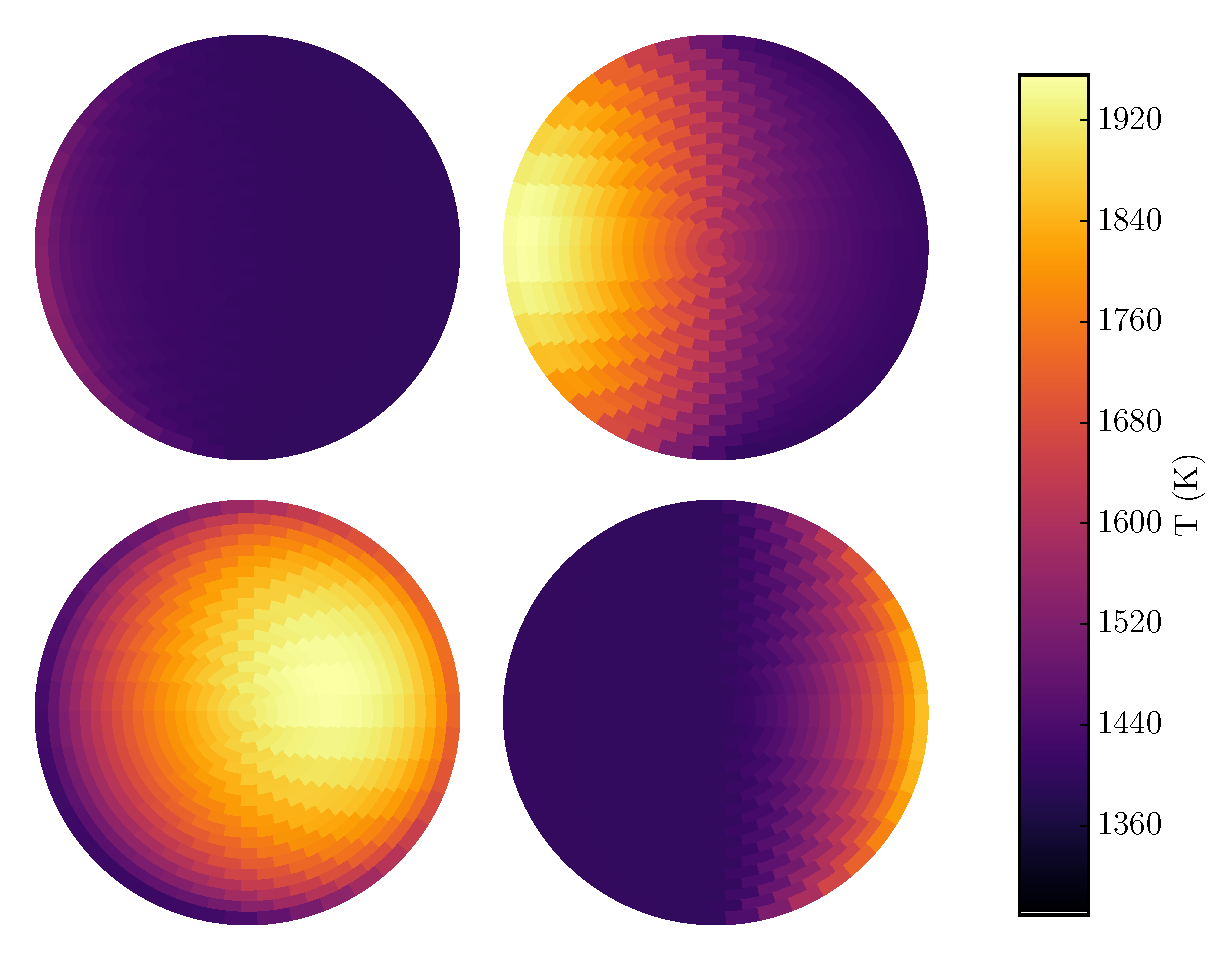
\includegraphics[width=\columnwidth]{img/free_parameterstemp_map.pdf}
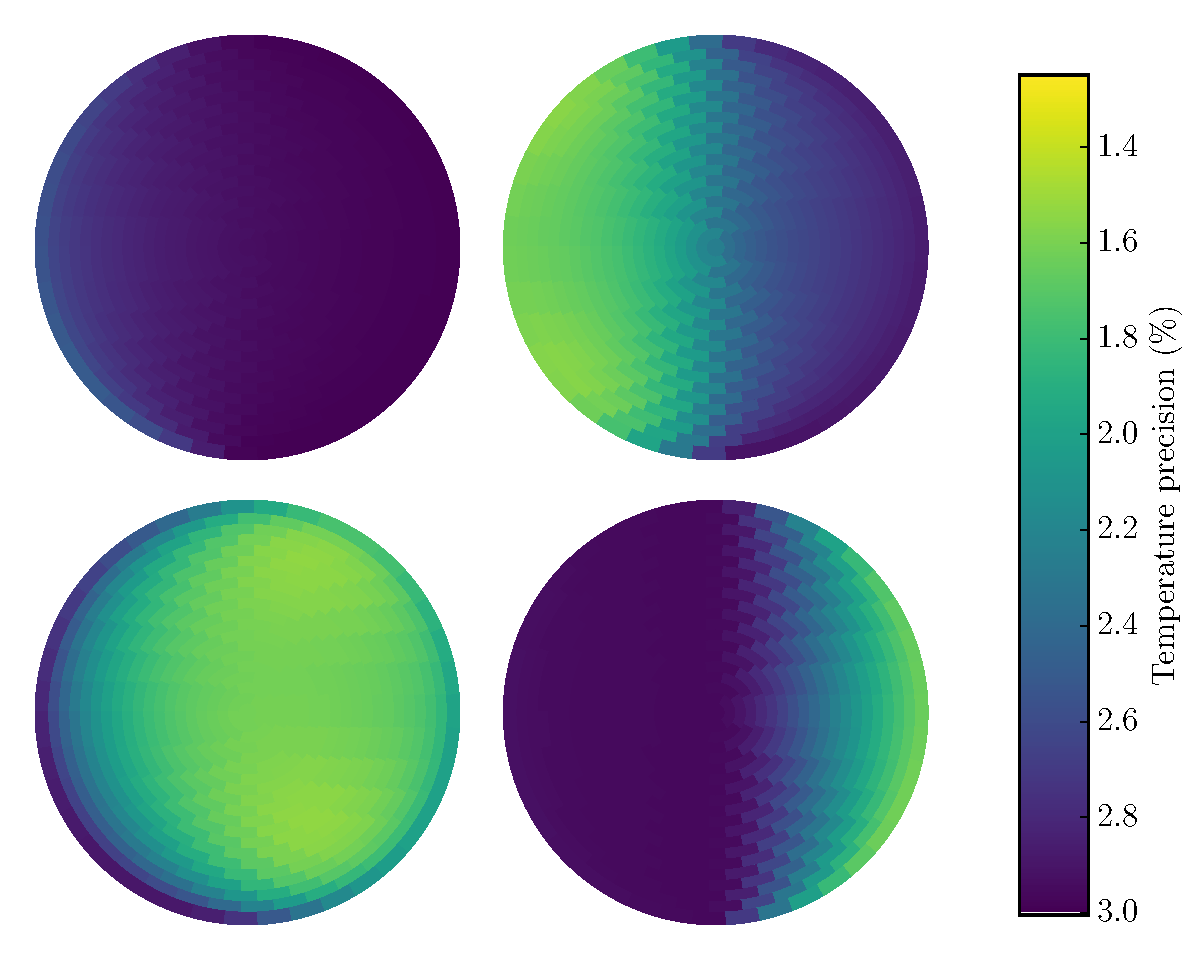
\includegraphics[width=\columnwidth]{img/free_parameterstemp_errs.pdf}
\caption{The underlying temperature distributions generated by the zhang model.}
\label{fig:best_fit_temp}
\end{center}
\end{figure*}

\begin{figure*}
\begin{center}
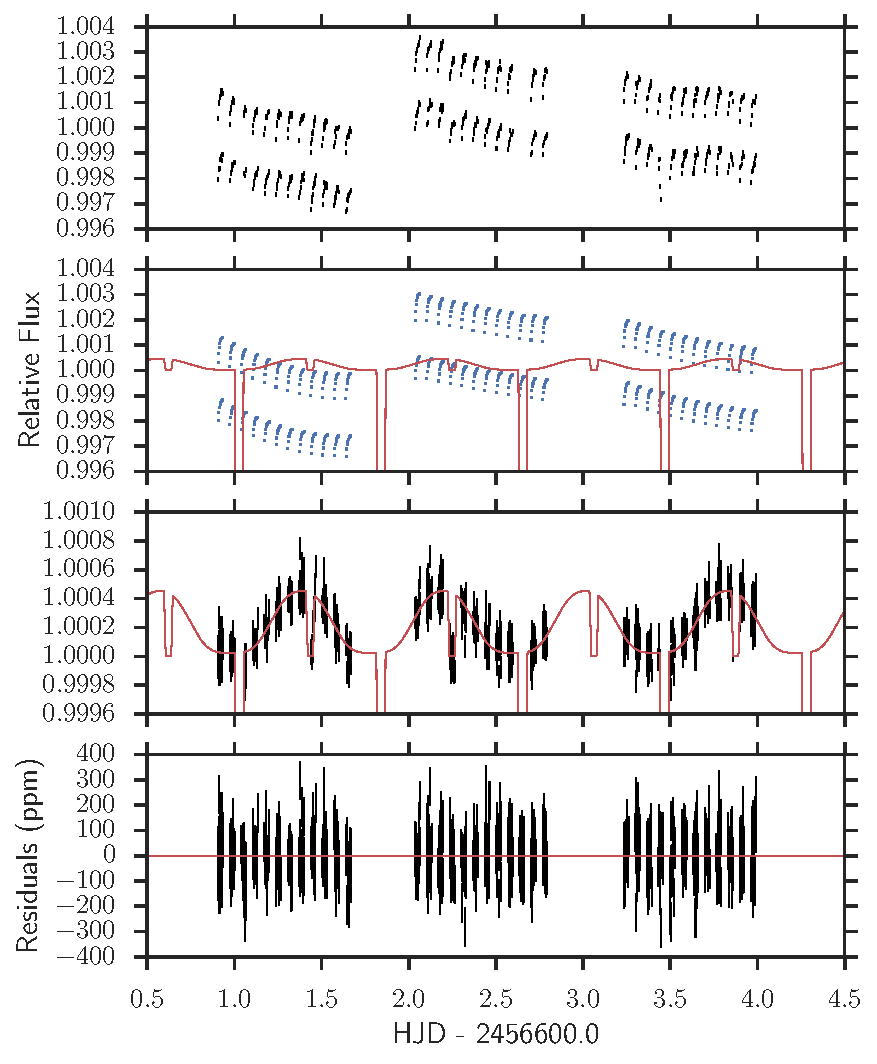
\includegraphics[width=1.0\textwidth]{img/systematics.pdf}
\caption{Top: raw data from HST, the systematic components are all visible. second panel shows the physical model fit (red) and the systematic model (blue). The third panel shows the model fit to the data with the systematic noise component removed, the fourth panel is the residuals of the fit.
}
\label{fig:systematics}
\end{center}
\end{figure*}

%\begin{figure*}
%\begin{center}
%\includegraphics[width=\textwidth]{img/huge_triangle.pdf}
%\caption{This triangle plot includes all the parameters that were used to fit the free limb darkening case.}
%\label{fig:big triangle}
%\end{center}
%\end{figure*}

\section*{Acknowledgements}

T.L. is supported by STFC consolidated grant (ST/L000733/1). Much of this work was carried out at the kavli summer program in physics 2016. T.L extends his gratitude to the program organisers, in particular Jonathan Fortney and Pascale Garaud.

%%%%%%%%%%%%%%%%%%%%%%%%%%%%%%%%%%%%%%%%%%%%%%%%%%

%%%%%%%%%%%%%%%%%%%% REFERENCES %%%%%%%%%%%%%%%%%%

% The best way to enter references is to use BibTeX:

\bibliographystyle{mnras}
%\bibliography{/home/astro/phrmat/Documents/BibTeX/Papers-LowEUV}
\bibliography{bibliography}
%\bibliography{example} % if your bibtex file is called example.bib


% Alternatively you could enter them by hand, like this:
% This method is tedious and prone to error if you have lots of references
%\begin{thebibliography}{99}
%\bibitem[\protect\citeauthoryear{Author}{2012}]{Author2012}
%Author A.~N., 2013, Journal of Improbable Astronomy, 1, 1
%\bibitem[\protect\citeauthoryear{Others}{2013}]{Others2013}
%Others S., 2012, Journal of Interesting Stuff, 17, 198
%\end{thebibliography}

%%%%%%%%%%%%%%%%%%%%%%%%%%%%%%%%%%%%%%%%%%%%%%%%%%

%%%%%%%%%%%%%%%%% APPENDICES %%%%%%%%%%%%%%%%%%%%%

%\appendix

%\section{Some extra material}

%If you want to present additional material which would interrupt the flow of %the main paper,
%it can be placed in an Appendix which appears after the list of references.

%%%%%%%%%%%%%%%%%%%%%%%%%%%%%%%%%%%%%%%%%%%%%%%%%%


% Don't change these lines
\bsp	% typesetting comment
\label{lastpage}
\end{document}

% End of mnras_template.tex